\documentclass{article}
\usepackage{tikz}
\usetikzlibrary{calc,intersections}
\usepackage{booktabs}
\usepackage{amsmath}
\begin{document}

\begin{figure}
    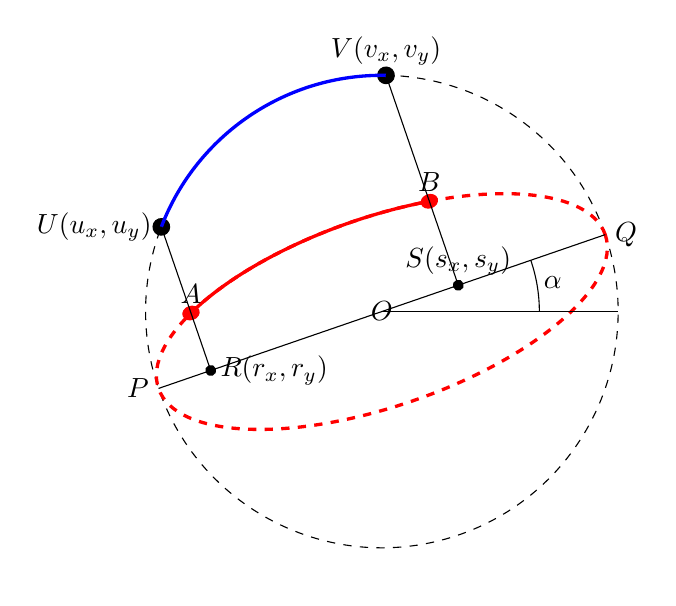
\begin{tikzpicture}
        \begin{scope}[rotate=19]
            \draw[dashed] (0,0) circle (3cm);
            \coordinate (Bc) at (70:3cm);
            \coordinate (Ac) at (140:3cm);
            \coordinate (P) at (-3,0);
            \coordinate (Q) at (3,0);
            \draw[fill] (Ac) circle (3pt);
            \draw[fill] (Bc) circle (3pt);
            \node at (Ac) [above,left] {$U(u_x,u_y)$};
            \node at (Bc) [above] {$V (v_x,v_y)$};
            \node at (P) [left] {$P$};
            \node at (Q) [right] {$Q$};
            \node at (0,0) {$O$};
            \draw[blue,very thick] (Bc) arc (70:140:3cm);
            \begin{scope}[yscale=0.4]
                \draw[very thick,red,dashed] (0,0) circle (3cm);
                \coordinate (Bm) at (70:3cm);
                \coordinate (Am) at (140:3cm);
                \draw[fill,red] (Am) ellipse (3pt and 6pt);
                \draw[fill,red] (Bm) ellipse (3pt and 6pt);
                \draw[red,very thick] (Bm) arc (70:140:3cm);
                \node at (Am) [above] {$A$};
                \node at (Bm) [above] {$B$};
            \end{scope}
            \draw[name path=lineA] (Am) -- (Ac);
            \draw[name path=lineB] (Bm) -- (Bc);
            \draw[name path=majorAxis] (P) -- (Q);
            \coordinate (Ax) at (intersection of Ac--Am and P--Q);
            \coordinate (Bx) at (intersection of Bc--Bm and P--Q);
            \fill (Ax) circle (2pt);
            \fill (Bx) circle (2pt);
            % \fill [blue, name ] circle (2pt);
            \draw (Am) -- (Ax);
            \draw (Bm) -- (Bx);
            \node at (Ax) [below,right] {$R (r_x,r_y)$};
            \node at (Bx) [above] {$S (s_x,s_y)$};
        \end{scope}
        \draw (0,0) -- (3,0);
        \draw (2,0) arc (0:19:2cm);
        \node at (9.5:2.2) {$\alpha$};
    \end{tikzpicture}
    \caption{The red arc $AB$ is a $y$-scaled copy of the blue arc $UV$.}
\end{figure}

\noindent
Given the positions $A$, $B$, and $M$ on the ideal unit
sphere, computed as outlined below, here are the steps to draw line segment $AB$:
\begin{enumerate}
    \item If $A$ and $M$ are not nearly antipodal (i.e. the angle between $A$ and $-M$ is bigger than $SETTINGS.nearlyAntipodalAngle$) then compute the cross product $\mathbf N = [N_x, N_y, N_z]$ of the vectors $A$ and $M$ to determine the normal vector to the plane containing the red circle (i.e. the plane containing $A$, $M$, $B$, and $O$). If $A$ and $M$ are nearly antipodal let $N = A \times B$.
    \item The major axis of the ellipse is the intersection of the plane containing the red circle and the
          $XY$ plane.  This means that in an orthogonal projection of the red circle plane onto the $XY$ plane the major axis of ellipse is in the direction $\mathbf{PQ} = [-N_{y}, N_{x}, 0]$
\end{enumerate}

Lines and line segments are managed as a \verb|Two.Group| of \verb|Two.Path|;
one path for the foreground semicircle and another path for the background
semicircle. The two semicircles are separated by the ellipse major axis.
This approach allows us to apply different visual styles to each semicircle.
In order to benefit from this organization, all drawing details must be
expressible in terms of the ellipse major and minor axes.

The red arc $AB$ is rendered by applying $y$-scale to the blue arc $UV$.
The $y$-scaling essentially projects $U$ and $V$ to $A$ and $B$ respectively,
using a projector line parallel to the minor axis
(hence perpendicular to the major axis).

Given the two mouse click positions $A$ and $B$, we can determine the locus
of $U$ and $V$ on the boundary circle using the following steps:

\begin{enumerate}
    \item Compute the normal vector of the plane containing the red circle,
          which is the cross product $\mathbf N = [N_x, N_y, N_z]$ of the normal vectors at $A$ and $B$.
    \item Since the ellipse major is on the $XY$ plane and is also $\perp$ to $\mathbf N$, we can fix the major axis direction $\vec{\mathbf {PQ}} = [-N_y, N_x, 0]$
    \item Determine the angle $\alpha$ between $PQ$ and the $X$-axis
    \item Rotate the entire diagram by $-\alpha$, so now:
          \begin{itemize}
              \item The major axis $PQ$ aligns with the $X$-axis
              \item All the projector lines $UA$ and $VB$ are parallel to the $Y$-axis
          \end{itemize}
          \textbf{After} this rotation by $-\alpha$ the following must be true: $a_x = r_x = u_x$  and $b_x = s_x = v_x$ and it is possible to determine the $x$-coordinates of $U$ and $V$ from the $x$-coordinates of the (rotated) mouse click positions.


    \item Since both $U$ and $V$ are on the unit circle, we can calculate the following quantities $u_y = \sqrt{(1 - u_x^2)}$ and $v_y = \sqrt{(1 - v_x^2)}$
    \item Determine the \verb|startAngle| ($\angle\; QOV$) and \verb|endAngle| ($\angle\; QOU$) and use these two values to determine which arc sections that must be rendered in foreground and background.
\end{enumerate}

This is going to be unstable if $A$ and $B$ are nearly antipodal and doesn't work if $A$ and $B$
are exactly antipodal.  This means that we need introduce a ``midpoint" of $A$ and $B$, called $M$,
that is dynamically updated as the user mouse downs (at $A$) and drags. The location of  $M$ \textbf{must be} constrained as the user mouse downs and drags. The location of the mouse moved (and potential mouse release location - i.e. $B$) event is \textbf{not} the location of $B$.

Let $A$ be the location in the unit sphere of the mouse down event. Initially, $M = A$. Now suppose that the user drags so that a mouse move event happens at location $C$ on the unit sphere. Let:
\begin{itemize}
    \item $B$ be the displayed endpoint of the drawn line segment (could be temporary or final if $C$ is also a mouse release point),
    \item $M_{old} = M$,
    \item $U = \frac{1}{2}(A+C))$ and $T= \frac{U}{|U|}$ ($T$ is the unit normalization of the midpoint of the line segment $AC$ that goes through the sphere), and
    \item  $\alpha = SETTINGS.maxMidpointMovementAngle$.
\end{itemize}
To compute $B$ and the new $M$ use the following:
\begin{itemize}
    \item If the angle between $T$ and $M_{old}$ is less than $\alpha$ then $B = C$ and $M = T$.
    \item If not then $M$ is the point on the circle of radius $\alpha$ about $M_{old}$ that is closest to $T$ and $B$ is the point so that if you normalize $\frac{1}{2} (A+B)$ you get the point $M$.\\ To compute $M$:
          \begin{enumerate}
              \item Let $F = M_{old} \times T$ and $G= F \times M_{old}$. (Notice that $F$, $G$, and $M_{old}$ form a unit orthogonal frame. To avoid numerical instability $F$ and $G$ might need to be normalized.)
              \item Then $M = \cos(\alpha)M_{old} + \sin(\alpha)G$
          \end{enumerate}
          To compute $B$:
          \begin{enumerate}
              \item Let $H= A \times M$ and $J = H \times A$. (Again notice that $H$, $J$, and $A$ form a unit orthogonal frame. To avoid numerical instability $H$ and $J$ might need to be normalized.)
              \item Let $\theta$ be the angle between $A$ and $M$, then $B = \cos(2\theta)A + \sin(2\theta)J$. (Again $B$ should be normalized.)
          \end{enumerate}
\end{itemize}




Each semicircle is rendered in CCW order which implies that $\text{startAngle} < \text{endAngle}$.

\begin{tabular}{cccc}
    \toprule
    \verb|startAngle| ($S$) & \verb|endAngle| ($E$) & Background                     & Foreground \\
    \midrule
    $S> 0$                       & $E> 0$                       & --                             & $[S,E]$    \\
    $S>0$                        & $E<0$                        & \multicolumn{2}{c}{impossible}              \\
    $S< 0$                       & $E> 0$                       & $[S,0]$                        & $[0,E]$    \\
    $S< 0$                       & $E< 0$                       & $[S,E]$                        & --         \\
    \bottomrule
\end{tabular}
\end{document}